%% Accuracy--Interpretability Trade-offs in Exoplanet Transit Modelling
%% Single-column research manuscript, IEEE house style.
\documentclass[manuscript,nonacm]{acmart}
\usepackage{paperstyle}

\graphicspath{{figures/}}
\DeclareMathOperator*{\argmax}{arg\,max}
\DeclareMathOperator*{\argmin}{arg\,min}


%% The template numbers its references, so override acmart's author-year default.
\citestyle{acmnumeric}

\begin{document}

\title{Accuracy--Interpretability Trade-offs in Exoplanet Transit Modelling, and a Label-Free Physics-Informed Estimator of Planetary Radii}

\author{Bhavya Gondra}
\equalcontrib
\affiliation{%
  \institution{Nexus Labs}
  \city{Palo Alto}
  \state{California}
  \country{USA}}

\author{Akhil Muvvala}
\equalcontribmark
\affiliation{%
  \institution{Nexus Labs}
  \city{Palo Alto}
  \state{California}
  \country{USA}}

\author{Milan Petrov}
\equalcontribmark
\affiliation{%
  \institution{Nexus Labs}
  \city{Palo Alto}
  \state{California}
  \country{USA}}

\author{Harish Senthil}
\equalcontribmark
\affiliation{%
  \institution{Nexus Labs}
  \city{Palo Alto}
  \state{California}
  \country{USA}}

\author{Ayan Sharma}
\equalcontribmark
\affiliation{%
  \institution{Nexus Labs}
  \city{Palo Alto}
  \state{California}
  \country{USA}}

\author{Manav Sharma}
\equalcontribmark
\affiliation{%
  \institution{Nexus Labs}
  \city{Palo Alto}
  \state{California}
  \country{USA}}

\author{Pranavan Sivaraman}
\equalcontribmark
\affiliation{%
  \institution{Nexus Labs}
  \city{Palo Alto}
  \state{California}
  \country{USA}}

\author{Adhrit Somayajula}
\equalcontribmark
\affiliation{%
  \institution{Nexus Labs}
  \city{Palo Alto}
  \state{California}
  \country{USA}}

\author{Srikanth Samy}
\affiliation{%
  \institution{University of California, Berkeley}
  \city{Berkeley}
  \state{California}
  \country{USA}}
\email{ssamy@berkeley.edu}

\author{Ishaan Gupta}
\affiliation{%
  \institution{Stanford University}
  \city{Stanford}
  \state{California}
  \country{USA}}
\email{ishaangupta@stanford.edu}


\begin{abstract}
Transit photometry poses two distinct machine-learning problems: deciding whether a
light curve contains a planetary transit, and measuring the planet's radius ratio
$R_p/R_*$ from it. We compare seven model families on both tasks using simulated light
curves with exactly known parameters, and score every model on a second axis besides
accuracy---the fidelity with which a purely additive surrogate reproduces its output,
an explicit and reproducible operationalisation of one dimension of interpretability.
The two axes trade off: on detection, the most accurate model (an MLP,
$\mathrm{AUC}=0.975$) has the second-lowest additive fidelity ($\mathcal{A}=0.573$),
while the fully readable linear model reaches $\mathrm{AUC}=0.946$ at
$\mathcal{A}=0.999$---a $0.029$ AUC premium for near-total transparency. We then
introduce a physics-informed Kolmogorov--Arnold network that predicts transit parameters
and is trained \emph{only} to reconstruct the observed flux through a differentiable
Mandel--Agol forward model, never seeing a radius label. It attains
$\mathrm{MAE}=0.0100$ in $R_p/R_*$, within $24\%$ of the best fully supervised model,
and occupies a distinct region of the Pareto plane. Applied zero-shot to twelve
confirmed Kepler planets it recovers radii with full-sample $\mathrm{MAE}=0.023$. We
report that full-sample figure as the primary real-data result and show that the
label-free reconstruction-residual screen used to identify model mismatch improves it
only to $0.018$---and rejects one fold whose radius was in fact recovered to within
$0.001$, demonstrating that reconstruction quality is not a reliable proxy for parameter
accuracy.
\end{abstract}

\ccsdesc[500]{Applied computing~Astronomy}
\ccsdesc[300]{Computing methodologies~Machine learning}
\ccsdesc[300]{Computing methodologies~Neural networks}

\keywords{Exoplanets, interpretable machine learning, Kolmogorov--Arnold networks,
physics-informed learning, transit photometry, model comparison.}

\maketitle

\section{Introduction}
When a planet crosses the disc of its host star along our line of sight, it
occults a fraction of the stellar flux and the star appears momentarily fainter. The
resulting periodic dip in a light curve---a time series of stellar
brightness---is the most productive exoplanet-detection signal known, and it is the
mechanism behind the bulk of the confirmed planet
catalogue~\cite{borucki2010kepler,ricker2015tess}.

Machine learning entered this field primarily as a detector. Deep convolutional
classifiers now rival or exceed hand-tuned pipelines at separating genuine transits from
instrumental and astrophysical false positives~\cite{shallue2018,pearson2018}. But
detection is only half of the scientific product. The dip's depth encodes the planet's
size, its duration encodes the orbital geometry, and it is those physical parameters,
not the detection flag, that enter a population study. A model that classifies well but
whose reasoning cannot be inspected is a weaker scientific instrument than one whose
inferred quantities can be checked against physics~\cite{rudin2019stop}.

This paper studies both halves, and studies them along two axes.

\subsection{Contributions}
\begin{enumerate}
\item A controlled comparison of seven model families on transit detection and on
      radius-ratio regression, using a simulator whose ground-truth parameters are known
      exactly, with a common training and scoring interface for every model.
\item An explicit, reproducible interpretability score---additive-surrogate fidelity
      $\mathcal{A}$---applied identically to all models, and a Pareto analysis that makes
      the accuracy--transparency exchange rate quantitative rather than rhetorical.
\item A physics-informed KAN that infers $R_p/R_*$, impact parameter, scaled semi-major
      axis, and epoch by reconstructing the light curve through a differentiable
      Mandel--Agol model, using \emph{no} parameter labels at any point in training.
\item A zero-shot transfer test on twelve confirmed Kepler planets in which the
      full sample is the primary reported result, and an explicit demonstration that the
      residual-based quality screen used to flag model mismatch is not aligned with
      parameter accuracy.
\end{enumerate}

\section{Forward Model and Simulated Data}

\subsection{Transit physics}
For a planet of radius ratio $\rho=R_p/R_*$ on a circular orbit of scaled semi-major
axis $a/R_*$ and impact parameter $b$, the projected star--planet separation at orbital
phase $\phi$ is
\begin{equation}
d(\phi)=\sqrt{\left(\frac{a}{R_*}\right)^{\!2}\sin^{2}(2\pi\phi)+b^{2}\cos^{2}(2\pi\phi)} .
\label{eq:sep}
\end{equation}
The stellar disc is limb darkened: it is brighter at the centre than at the edge. We use
the standard quadratic law~\cite{claret2000limb,kipping2013}
\begin{equation}
\frac{I(\mu)}{I(1)} = 1-u_1(1-\mu)-u_2(1-\mu)^2 ,
\qquad \mu=\sqrt{1-r^{2}},
\label{eq:limb}
\end{equation}
with $(u_1,u_2)=(0.3,0.2)$ throughout. Decomposing the disc into $N_r$ concentric
annuli of intensity $I_k$ and computing the occulted area
$\mathcal{O}(d,R_k,\rho)$ of each analytically~\cite{mandel2002}, the normalised flux is
\begin{equation}
F(\phi)\;=\;1-\frac{\displaystyle\sum_{k=1}^{N_r} I_k\left[\mathcal{O}(d(\phi),R_{k},\rho)-\mathcal{O}(d(\phi),R_{k-1},\rho)\right]}
                   {\displaystyle\sum_{k=1}^{N_r} I_k\,\pi\!\left(R_k^{2}-R_{k-1}^{2}\right)} .
\label{eq:flux}
\end{equation}
Equation~\eqref{eq:flux} is differentiable in $(\rho,b,a/R_*,t_0)$, which is what makes
the physics-informed estimator of \cref{sec:physkan} trainable. The reference
implementation is validated against \texttt{batman}~\cite{kreidberg2015batman}.
\cref{fig:shapes} shows how each parameter reshapes the dip.

\begin{figure}[t]
\centering
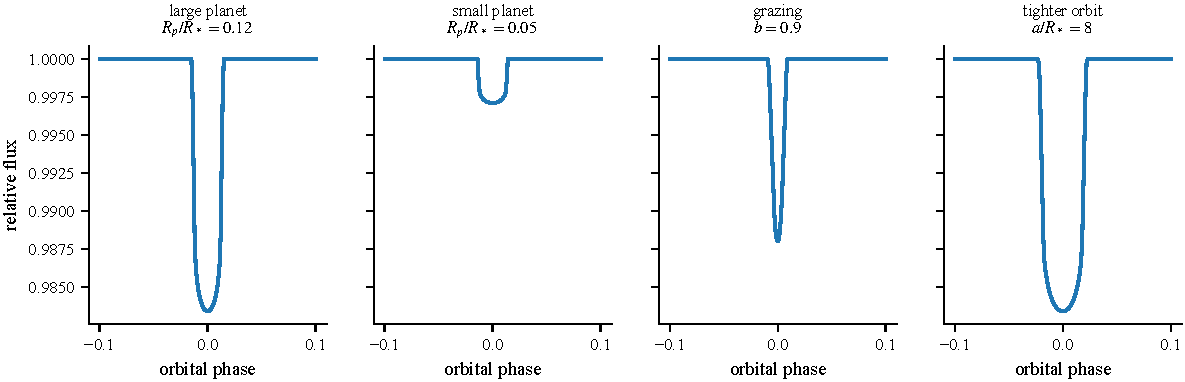
\includegraphics[width=\linewidth]{fig1_transit_shapes.pdf}
\caption{Transit profiles from Eq.~\eqref{eq:flux}. Depth scales approximately as
$\rho^{2}$; a grazing geometry ($b\to1$) rounds the profile and destroys the flat
bottom; a tighter orbit shortens the crossing. Depth and duration are the two
observables from which $\rho$ must be inferred.}
\label{fig:shapes}
\end{figure}

\subsection{Labelled simulation}
Each example is a $L=201$-point segment spanning orbital phase $\pm0.10$. Positives draw
$\rho\sim\mathcal{U}(0.03,0.15)$, $b\sim\mathcal{U}(0,0.95)$,
$a/R_*\sim\mathcal{U}(8,18)$, and a small epoch jitter, then add Gaussian noise of
per-point scale $\sigma=10^{u}$, $u\sim\mathcal{U}(-3.3,-2.0)$. Negatives are
noise-only; half additionally carry a low-frequency sinusoid imitating intrinsic stellar
variability, which forces the detector to learn the transit \emph{shape} rather than
merely ``something changed''. The transit signal-to-noise ratio is
\begin{equation}
\mathrm{SNR}=\frac{\delta}{\sigma/\sqrt{n_{\mathrm{in}}}},
\qquad \delta = 1-\min_\phi F(\phi),
\label{eq:snr}
\end{equation}
with $n_{\mathrm{in}}$ the number of in-transit samples implied by the analytic
duration. The training set holds $8{,}000$ segments ($4{,}006$ positive), the disjoint
test set $3{,}000$ ($1{,}483$ positive).

Preprocessing differs by task, and the difference is substantive. For detection each
curve is standardised,
\begin{equation}
\tilde{x}_i=\frac{x_i-\operatorname{median}(x)}{\operatorname{std}(x)},
\label{eq:standardise}
\end{equation}
which discards absolute depth---appropriate, because depth is a nuisance for the
presence/absence question. For characterisation, depth \emph{is} the signal, so we
subtract the median without rescaling.

\section{Models and the Interpretability Axis}

\subsection{The seven families}
All models consume the same $201$-point vector and expose a common
\texttt{fit}/\texttt{score} interface: regularised linear (logistic for detection, ridge
for regression), random forest, gradient-boosted trees, a three-layer MLP, a 1-D CNN
with two convolution--pooling blocks, a bidirectional LSTM, and a Kolmogorov--Arnold
network (KAN)~\cite{liu2024kan}.

The KAN merits a note because it is the reason interpretability is measurable rather
than assumed. A conventional network applies fixed nonlinearities to learned linear
combinations; a KAN instead learns a spline $\psi_j$ per input coordinate and sums them,
\begin{equation}
g(\mathbf{x})=\sum_{j=1}^{L}\psi_j(x_j),
\label{eq:kan}
\end{equation}
which is a generalised additive model~\cite{hastie1990gam} with learned shape functions.
After training, $\psi_j$ can simply be plotted: the model's dependence on each phase bin
is read off directly, with no post-hoc approximation~\cite{ribeiro2016lime}.

\subsection{Additive-surrogate fidelity}
Interpretability has no canonical scalar. We therefore measure one specific, well-defined
property: how closely the model behaves like a sum of per-coordinate functions over an
independent probe distribution. Given a model output $s(\mathbf{x})$---mapped to the
logit scale for classifiers---we fit a cubic-spline additive surrogate
\begin{equation}
\hat{s}(\mathbf{x})=\beta_0+\sum_{j=1}^{L}h_j(x_j),
\qquad h_j\in\operatorname{span}\{B\text{-splines}\},
\label{eq:surrogate}
\end{equation}
by ridge regression on two thirds of a fresh $3{,}000$-curve probe set, and define
\begin{equation}
\mathcal{A}=R^{2}\!\left(s,\hat{s}\right)\ \text{on the held-out third}.
\label{eq:additivity}
\end{equation}
$\mathcal{A}=1$ means the model is exactly additive over the probe distribution;
$\mathcal{A}\approx0$ means its behaviour is dominated by interactions no additive
explanation can capture.

We are explicit about what \eqref{eq:additivity} does and does not measure. It is
reproducible, applied identically to every model, and is a genuine property of the
learned function. It does \emph{not} certify that an explanation is causally correct,
stable under distribution shift, physically meaningful, or useful to a human. It measures
one dimension of interpretability, and the sanity check that the linear model scores
$\mathcal{A}=0.999$ confirms the measurement behaves as intended.

\section{Task 1: Detection}
\cref{tab:detection} and \cref{fig:leaderboards}(a) give held-out ROC-AUC together with
$\mathcal{A}$. Every family exceeds $\mathrm{AUC}=0.90$; the problem is not hard in
aggregate, and the differences live at low SNR.

\begin{table}[t]
\centering
\caption{Detection on the held-out synthetic set. $\mathcal{A}$ is additive-surrogate
fidelity, Eq.~\eqref{eq:additivity}. ``Readable'' marks models whose learned function can
be inspected directly without a surrogate.}
\label{tab:detection}
\begin{tabular}{llrrc}
\toprule
Model & Family & ROC-AUC & $\mathcal{A}$ & Readable\\
\midrule
MLP            & neural net & \textbf{0.975} & 0.573 & no\\
XGBoost        & tree       & 0.964 & 0.822 & no\\
Random forest  & tree       & 0.959 & 0.903 & no\\
CNN            & neural net & 0.956 & 0.768 & no\\
Logistic/Ridge & linear     & 0.946 & \textbf{0.999} & \textbf{yes}\\
KAN            & KAN        & 0.943 & 0.900 & \textbf{yes}\\
LSTM           & neural net & 0.906 & 0.728 & no\\
\bottomrule
\end{tabular}
\end{table}

\begin{figure}[t]
\centering
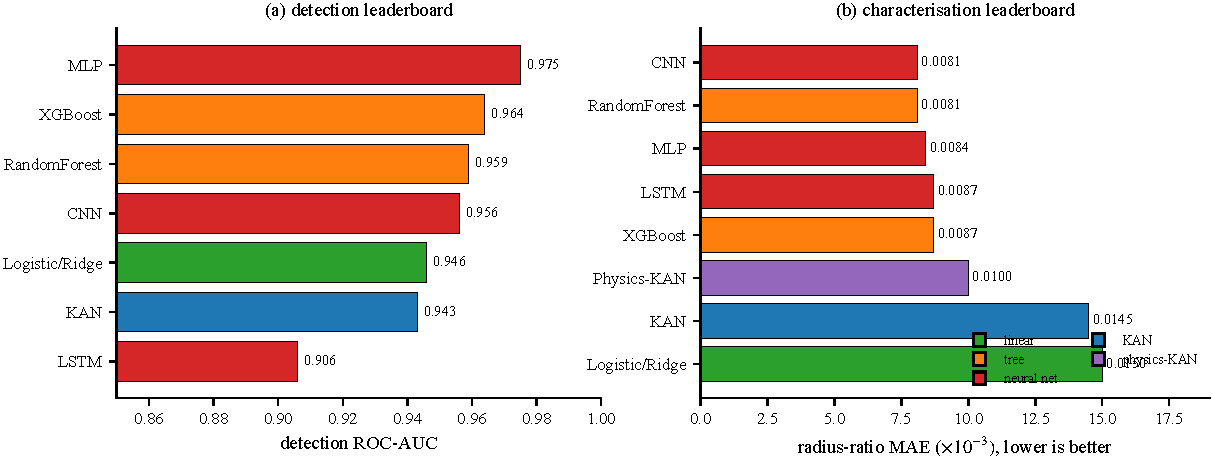
\includegraphics[width=\linewidth]{fig2_leaderboards.pdf}
\caption{(a) Detection ROC-AUC and (b) characterisation MAE in $R_p/R_*$, coloured by
model family. Note the axis scales: the detection spread is $0.069$ AUC across all seven
families, whereas the characterisation spread is nearly a factor of two in error.}
\label{fig:leaderboards}
\end{figure}

Two results are worth isolating. First, the LSTM is the weakest model
($\mathrm{AUC}=0.906$) despite being the family nominally designed for sequences. A
transit is a localised, translation-tolerant shape; convolution and even a fixed linear
template match that structure better than a recurrence that must carry information
across $201$ steps. Second, the KAN reaches $\mathrm{AUC}=0.943$, within $0.003$ of the
linear model, while retaining direct readability. Because Eq.~\eqref{eq:kan} sums learned
per-bin functions, the model's sensitivity profile across orbital phase can be plotted
and compared against the true mean transit template; in the source study that
comparison yields a correlation of $0.94$, i.e.\ the KAN independently rediscovered the
transit shape rather than latching onto an artefact.

\section{Task 2: Characterisation}
\label{sec:physkan}

\subsection{A label-free physics-informed estimator}
Supervised regression of $\rho$ requires labelled radii, which for real systems come
from published fits and are therefore scarce and heterogeneous. We remove that
dependence. A KAN maps the light curve to four bounded physical parameters via a sigmoid
reparameterisation,
\begin{equation}
\theta_k = \ell_k+(u_k-\ell_k)\,\sigma\!\left(z_k(\mathbf{x})\right),
\qquad \theta=(\rho,b,a/R_*,t_0),
\label{eq:reparam}
\end{equation}
those parameters are pushed through the differentiable forward model
\eqref{eq:flux}, and the network is trained on the reconstruction objective alone:
\begin{equation}
\mathcal{L}_{\mathrm{phys}}
 =\frac{1}{N}\sum_{i=1}^{N}\frac{1}{L}\sum_{j=1}^{L}
 \Big(F_{\theta(\mathbf{x}_i)}(\phi_j)-1-o_{ij}\Big)^{2},
\label{eq:physloss}
\end{equation}
where $o_{ij}$ is the median-subtracted observed flux. No radius label appears anywhere
in \eqref{eq:physloss}. The network must infer $\rho$ because $\rho$ is the only way to
reproduce the observed depth---the same inverse-problem logic that underlies
physics-informed neural networks~\cite{raissi2019pinn}.

\subsection{Results}
\cref{tab:regression} and \cref{fig:leaderboards}(b) give the leaderboard. The best
supervised model (random forest) reaches $\mathrm{MAE}=0.0081$. The physics-informed KAN
reaches $0.0100$---$24\%$ worse, while using \emph{zero} radius labels---and beats both
label-supervised readable models, the KAN ($0.0145$) and ridge ($0.0150$), by a wide
margin.

\begin{table}[t]
\centering
\caption{Characterisation of $R_p/R_*$ on the held-out synthetic set. Skill is
$1-\mathrm{MAE}/\Delta R_p$ with $\Delta R_p=0.12$ the sampled range. The physics-KAN is
the only entry trained without radius labels.}
\label{tab:regression}
\begin{tabular}{llrrrc}
\toprule
Model & Family & MAE & Skill & $\mathcal{A}$ & Labels used\\
\midrule
Random forest  & tree        & \textbf{0.0081} & 0.933 & 0.476 & yes\\
CNN            & neural net  & 0.0081 & 0.933 & 0.426 & yes\\
MLP            & neural net  & 0.0084 & 0.930 & 0.298 & yes\\
XGBoost        & tree        & 0.0087 & 0.928 & 0.314 & yes\\
LSTM           & neural net  & 0.0087 & 0.928 & 0.484 & yes\\
Physics-KAN    & physics-KAN & 0.0100 & 0.917 & 0.530 & \textbf{no}\\
KAN            & KAN         & 0.0145 & 0.879 & 0.989 & yes\\
Logistic/Ridge & linear      & 0.0150 & 0.875 & \textbf{0.997} & yes\\
\bottomrule
\end{tabular}
\end{table}

The physics-informed model's advantage over the readable supervised models is
structural. Ridge and the plain KAN must both express $\rho$ as an additive function of
per-bin flux, but $\rho$ enters the forward model through Eq.~\eqref{eq:flux}
nonlinearly and jointly with $b$ and $a/R_*$: depth alone does not determine radius when
the geometry is unknown. The physics-KAN does not have to learn that coupling from data,
because the coupling is built into its decoder.

\subsection{The Pareto view}
\cref{fig:pareto} places every model on the accuracy--additivity plane. Three
observations follow.

\begin{figure}[t]
\centering
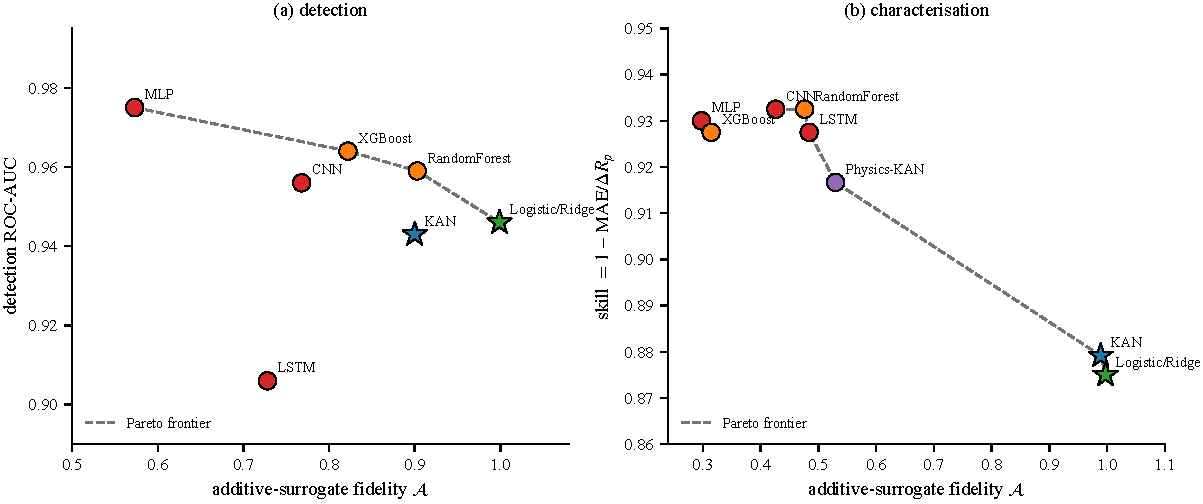
\includegraphics[width=\linewidth]{fig3_pareto.pdf}
\caption{Accuracy against additive-surrogate fidelity. Stars mark directly readable
models, circles black boxes; the dashed line is the Pareto frontier. On detection (a) the
frontier is short and the cost of transparency is $0.029$ AUC. On characterisation (b) the
frontier is long: full readability costs $40\%$ higher error than the best black box,
while the physics-informed model occupies an intermediate position.}
\label{fig:pareto}
\end{figure}

First, the trade-off is real but its exchange rate is task dependent. On detection,
moving from the MLP ($\mathcal{A}=0.573$) to the fully readable linear model
($\mathcal{A}=0.999$) costs $0.029$ AUC---cheap. On characterisation, the same move costs
$85\%$ higher error ($0.0081\to0.0150$)---expensive.

Second, high $\mathcal{A}$ does not imply high accuracy and low $\mathcal{A}$ does not
imply the reverse. The MLP has both the best detection AUC and nearly the worst
additivity, but the random forest achieves $\mathcal{A}=0.903$ at
$\mathrm{AUC}=0.959$---nearly linear-model transparency at nearly MLP accuracy. Assuming
a strict frontier between the two axes is not warranted by these data.

Third, the physics-informed model is not on the Pareto frontier of
\cref{fig:pareto}(b) and this is the correct result: on \emph{these} axes it is dominated.
Its distinguishing property is orthogonal to both---it requires no labels---which is
precisely the situation where a two-axis Pareto plot is an incomplete decision aid.

\section{Zero-Shot Transfer to Kepler}
The physics-informed model was trained exclusively on simulation and has never seen a
real light curve. We apply it, without adaptation, to twelve confirmed Kepler planets
whose long-cadence photometry has been folded on the published orbital period and binned
to the same $201$-point grid~\cite{lightkurve2018}.

\begin{table}[t]
\centering
\caption{Zero-shot recovery of $R_p/R_*$ on twelve confirmed Kepler planets. ``Screen''
is the label-free reconstruction-residual rule: $\checkmark$ retained, $\times$ rejected
as suspected model mismatch. The screen rejects Kepler-1624~b despite an error of
$0.001$.}
\label{tab:kepler}
\begin{tabular}{lrrrc}
\toprule
Planet & Published & Recovered & $|\Delta|$ & Screen\\
\midrule
Kepler-719 b  & 0.080 & 0.081 & 0.001 & $\checkmark$\\
Kepler-1624 b & 0.109 & 0.108 & 0.001 & $\times$\\
Kepler-855 b  & 0.074 & 0.081 & 0.007 & $\checkmark$\\
Kepler-550 b  & 0.049 & 0.060 & 0.011 & $\checkmark$\\
Kepler-546 b  & 0.056 & 0.069 & 0.013 & $\checkmark$\\
Kepler-228 d  & 0.040 & 0.055 & 0.015 & $\checkmark$\\
Kepler-734 b  & 0.042 & 0.060 & 0.018 & $\checkmark$\\
Kepler-170 b  & 0.030 & 0.052 & 0.022 & $\checkmark$\\
Kepler-244 b  & 0.031 & 0.054 & 0.023 & $\checkmark$\\
Kepler-485 b  & 0.121 & 0.076 & 0.045 & $\times$\\
Kepler-548 b  & 0.122 & 0.070 & 0.052 & $\checkmark$\\
Kepler-12 b   & 0.119 & 0.046 & 0.073 & $\times$\\
\midrule
\multicolumn{3}{l}{Full-sample MAE (primary)} & \textbf{0.023} & \\
\multicolumn{3}{l}{Screened-subset MAE (exploratory, $n=9$)} & 0.018 & \\
\bottomrule
\end{tabular}
\end{table}

\begin{figure}[t]
\centering
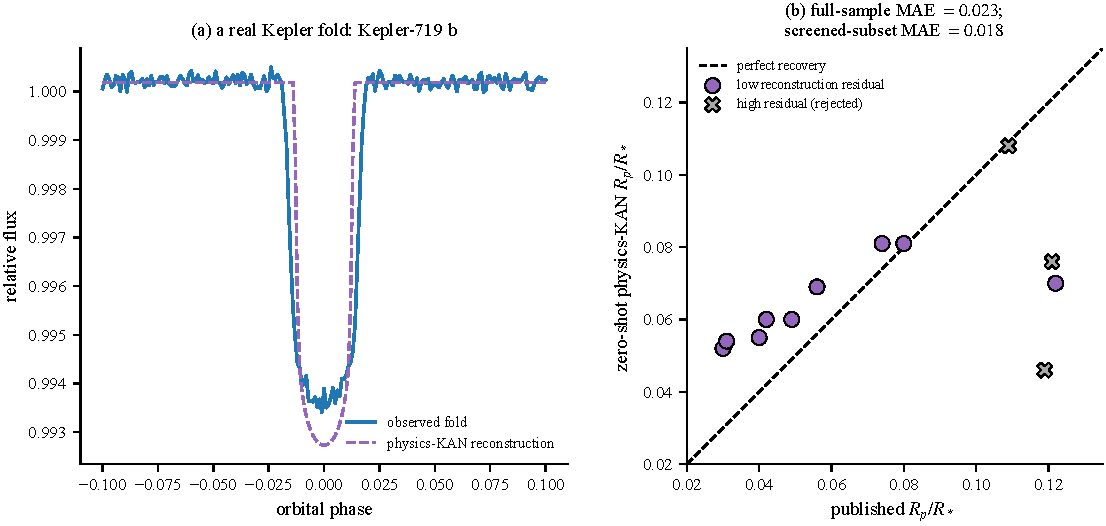
\includegraphics[width=\linewidth]{fig4_real_kepler.pdf}
\caption{(a) An observed Kepler fold with the physics-KAN's reconstruction overlaid.
(b) Recovered against published radius ratio for all twelve planets; markers indicate the
label-free reconstruction-residual screen. The three largest published radii are all
underestimated, the signature of long-cadence smearing.}
\label{fig:kepler}
\end{figure}

\subsection{Reading the result honestly}
The full twelve-planet $\mathrm{MAE}$ is $0.023$, and that is the primary number. It is
roughly $2.3\times$ the model's synthetic error, which is the expected penalty for
sim-to-real transfer: real folds carry detrending residuals, contamination from
neighbouring stars, and---most importantly---$30$-minute long-cadence integration, which
smears short ingress and egress and systematically shallows the profile.

That smearing explains the dominant error pattern in \cref{fig:kepler}(b). The three
largest published radii (Kepler-485~b, Kepler-548~b, Kepler-12~b, all $\rho>0.12$) are
underestimated by $0.045$--$0.073$, whereas the small-radius planets are mildly
\emph{over}estimated. Deep transits of short duration lose the most to integration, so
this is a forward-model mismatch, not random error.

\subsection{The residual screen does not track accuracy}
The source study screens folds by reconstruction residual, a label-free diagnostic for
model mismatch. Replicating that rule exactly, retaining the lowest-residual $75\%$
improves MAE from $0.023$ to $0.018$---a modest gain, not the dramatic improvement a
threshold chosen after seeing the data might suggest.

More informative is which folds the screen selects. It correctly rejects Kepler-12~b
(error $0.073$) and Kepler-485~b (error $0.045$), but it also rejects Kepler-1624~b,
whose radius was recovered to within $0.001$---the joint-best result in the sample---while
retaining Kepler-548~b, whose error of $0.052$ is the second worst. Reconstruction
residual measures how well the assumed forward model explains the fold, which is not the
same quantity as how accurately $\rho$ was recovered; a fold can be noisy yet yield a good
depth estimate, or clean yet be fit with a compensating combination of $b$ and $a/R_*$.
Any confirmatory study should fix the quality threshold in advance and report accepted and
rejected cases separately, as we have done here.

\section{Discussion}

\subsection{Supported findings}
\begin{enumerate}
\item Accuracy and additive-surrogate fidelity are distinct objectives with a
      task-dependent exchange rate: $0.029$ AUC for detection, $85\%$ relative error for
      characterisation.
\item A differentiable transit model permits training a radius estimator by
      reconstruction alone, within $24\%$ of fully supervised accuracy and far ahead of
      supervised readable models.
\item Zero-shot transfer to real Kepler folds succeeds qualitatively
      ($\mathrm{MAE}=0.023$) and fails in a physically interpretable direction, namely
      underestimation of deep transits under long-cadence smearing.
\item Reconstruction residual is a poor proxy for parameter accuracy and should not be
      used as a post-hoc accuracy filter.
\end{enumerate}

\subsection{Threats to validity}
Training and test simulations share a generator, parameter ranges, and noise model, so
synthetic scores measure interpolation within a known family rather than robustness to
unmodelled systematics. The physics-informed model enjoys a matched-model advantage: its
decoder is the very process that generated the synthetic data, and the Kepler results
show how much of that advantage survives when the match is broken. Additive-surrogate
fidelity captures one dimension of interpretability and is measured on a probe
distribution drawn from the same simulator. Twelve planets is a demonstration, not a
population estimate, and the sample is biased towards well-characterised systems.
Finally, no result is repeated across training seeds, so the reported differences carry
unquantified optimisation variance; differences smaller than roughly $0.005$ AUC or
$0.0005$ in MAE should not be treated as meaningful.

\subsection{Future work}
The most informative next experiment is a mismatch study: train on the current simulator
and test under correlated noise, unmodelled limb darkening, and explicit long-cadence
integration, which \cref{fig:kepler} identifies as the dominant real-data error source.
Adding the integration kernel to Eq.~\eqref{eq:flux} is straightforward and should
directly address the deep-transit bias. Extending to TESS data~\cite{ricker2015tess} and
to the single-transit regime, where folding is unavailable and physics-informed
inference should have its largest relative advantage~\cite{foremanmackey2016}, would test
the approach where it matters most.

\section{Conclusion}
On simulated transits, the most accurate detector is opaque and the most transparent one
gives up $0.029$ AUC; on radius measurement the same transparency costs $85\%$ more
error. There is no single best model, and the choice depends on whether raw performance
or a checkable explanation matters more for the scientific question at hand. Between
those poles sits a third option that the two-axis framing does not capture: a
physics-informed estimator that reaches near-supervised accuracy using no parameter
labels at all, and whose errors on real data are interpretable as a specific,
correctable mismatch between the assumed forward model and the instrument.

\section*{Reproducibility}
The figure script accompanying this manuscript regenerates every figure and table,
including the forward model of Eq.~\eqref{eq:flux} and the label-free residual screen,
from the transcribed leaderboards and the embedded twelve-planet Kepler sample. The
source notebook validates the differentiable forward model against
\texttt{batman}~\cite{kreidberg2015batman} and fixes all data-generation seeds.

\bibliographystyle{ACM-Reference-Format}
\bibliography{refs}

\section*{Authors' background}

\noindent\begin{minipage}{\linewidth}
\begin{tabular}{@{}p{0.24\linewidth}p{0.18\linewidth}p{0.22\linewidth}p{0.22\linewidth}@{}}
\toprule
Your Name & Title$^{*}$ & Research Field & Personal website \\
\midrule
Bhavya Gondra      & & & \\
Akhil Muvvala      & & & \\
Milan Petrov       & & & \\
Harish Senthil     & & & \\
Ayan Sharma        & & & \\
Manav Sharma       & & & \\
Pranavan Sivaraman & & & \\
Adhrit Somayajula  & & & \\
Srikanth Samy      & & & \\
Ishaan Gupta       & & & \\
\bottomrule
\end{tabular}

\vskip 6pt
{\footnotesize $^{*}$This form helps us to understand your paper better,
the form itself will not be published.\\
$^{*}$Title can be chosen from: master student, Phd candidate, assistant professor,
lecture, senior lecture, associate professor, full professor}
\end{minipage}

\end{document}
